\capitulo{6}{Trabajos relacionados}

\section{Similitud de Audio Mediante Redes Neuronales Siamesas}

\begin{figure}
    \centering
    \centerfloat
    \label{fig:siamese}
    \makebox[\textwidth][c]{%
    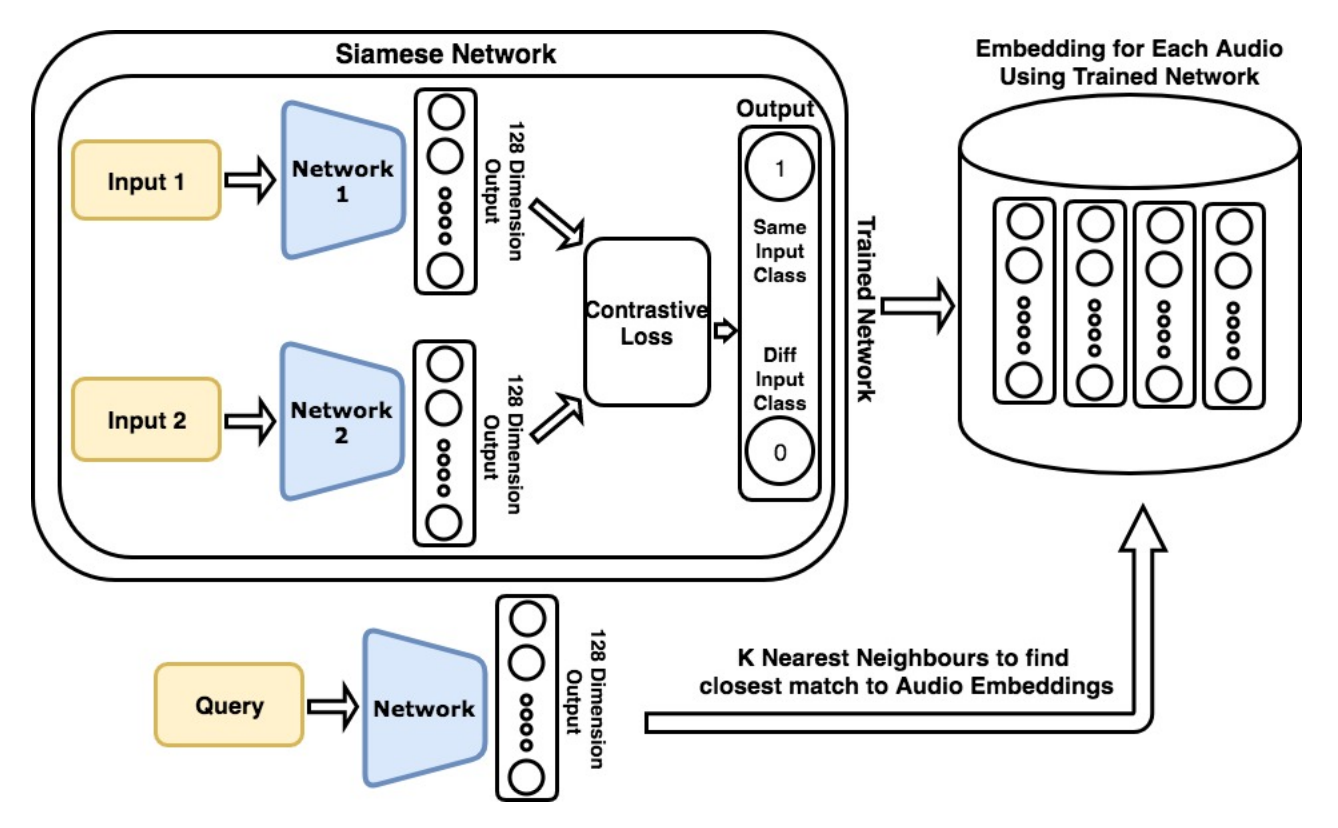
\includegraphics[width=1.2\textwidth]{img/6/siamese.png}%
    }
    
    \caption{Sistema de Recomendación basado en RNS. Extraído de \cite{siamese}}
    \label{fig:my_label}
\end{figure}

En \cite{siamese} presentan una aproximación mucho más interesante a la hora de calcular la similitud entre dos canciones usando redes neuronales siamesas. Este sistema utiliza dos redes neuronales exactamente iguales\footnote{misma arquitectura y pesos} Fig.\ref{fig:siamese}, con la que se obtiene una salida de 128 elementos. Esta salida es comparada mediante una función de pérdida que permite obtener la diferencia entre cada una de las entradas de la red. Se ha descartado esta aproximación de similitud por varias razones.\\
\\
\textbf{Entrenamiento:} Para poder entrenar una red siamesa es necesario agrupar manualmente los datos según su similitud. Cada grupo deben contener $N$ canciones similares y $N$ canciones diferentes.\footnote{N puede ser un número pequeño, de 4 o 5 canciones}\\
\textbf{Inferencia:} Para poder obtener la similitud de una canción es necesario comparar la salida de la red con todas las canciones mediante la función de comparación.


\section{Servicios Similares}

\subsection{Spotify}
Desde el inicio del proyecto, Spotify \cite{spotify} ha añadido algunas funcionalidades que se asemejan a las implementadas en este proyecto. Por un lado, Spotify ha añadido un sistema para rellenar playlists con canciones recomendadas, similar al sistema de recomendación de SpotMyFM. Por otro lado, Spotify crea periódicamente playlists personalizadas sobre un tema específico, como por el ejemplo \textbf{géneros}, \textbf{décadas}, \textbf{estados de ánimo} o \textbf{artistas}. Estas playlists están formadas por canciones de la biblioteca del usuario, así como recomendaciones.

\subsection{Rate Your Music}
Rate Your Music \cite{RYM} (RYM) es una plataforma colaborativa destinada a la clasificación y calificación de música. RYM no tiene integración con Spotify, pero gracias a su base de datos se incluyen características similares a SpotMyFM, como el poder etiquetar álbumes y añadir filtros a nivel de etiquetas, géneros o fechas. Por otro lado, RYM incluye un sistema de recomendación basado en las calificaciones del usuario. Este sistema de recomendación colaborativo, al igual que el que se ha planteado para SpotMyFM, no funciona a tiempo real.


\subsection{Obscurify}
Obscurify \cite{Obscurif67:online} es una web de código abierto que permite consultar las estadísticas personales de Spotify de manera similar a SpotMyFM. La principal diferencia entre Obscurify y SpotMyFM es que Obscurify únicamente muestra las estadísticas de artistas y canciones más escuchados durante el \textbf{último mes}, \textbf{último medio año} y \textbf{desde el inicio}, mientras que SpotMyFM permite consultar las estadísticas de dichos intervalos, la biblioteca completa del usuario y playlists individuales.

Obscurify está centrada en el análisis de popularidad de una biblioteca, y realiza este análisis a partir de una métrica que tienen en cuenta la popularidad de una canción o artistas, así como su posición en el top personal del usuario. Obscurify, a diferencia de SpotMyFM, no está centrado en la gestión de la biblioteca. 

La tabla \ref{tabla:obscurify} contiene una comparativa entre las funcionalidades de análisis de SpotMyFM y Obscurify. 


\begin{table}[]
\label{tabla:obscurify}
\caption{Comparativa entre Obscurify y SpotMyFM}
\resizebox{\textwidth}{!}{%
\begin{tabular}{@{}lll@{}}
\toprule
Funcionalidad                                                                             & SpotMyFM                                                                                  & Obscurify                               \\ \midrule
Alcance del Análisis                                                                      & \begin{tabular}[c]{@{}l@{}}Biblioteca\\ Playlists\\ Canciones más escuchadas\end{tabular} & Canciones más escuchadas                \\
Géneros Favoritos                                                                         & Si                                                                                        & Si                                      \\
\begin{tabular}[c]{@{}l@{}}Valoración General \\ de Popularidad\end{tabular}              & No                                                                                        & Si                                      \\
\begin{tabular}[c]{@{}l@{}}Canciones/Artistas\\ Menos Populares\end{tabular}              & Si (Métrica de Spotify)                                                                   & Si (Métrica especial)                   \\
\begin{tabular}[c]{@{}l@{}}Canciones/Artistas\\ Más Populares\end{tabular}                & Si                                                                                        & No                                      \\
Artistas Favoritos                                                                        & Si (Siempre)                                                                              & Si (último mes)                         \\
Agrupamiento por Décadas                                                                  & Si                                                                                        & Si                                      \\
Recomendaciones                                                                           & Si (Contenido)                                                                            & Si (Colaborativo)                       \\
Estados de Ánimo                                                                          & Si (análisis de la canción)                                                               & Parcial (Felicidad, Energía y Acústico) \\
\begin{tabular}[c]{@{}l@{}}Evolución de  los géneros\\ a lo largo del tiempo\end{tabular} & Si                                                                                        & No                                      \\
Filtros                                                                                   & Si                                                                                        & No                                      \\
Creación de Playlists                                                                     & Si (Cualquier Item)                                                                       & Si (Solo recomendaciones)                                      \\
Integración con LastFM                                                                    & Si                                                                                        & No                                      \\
Detalles de canciones / Artistas                                                          & Si                                                                                        & No                                      \\ \bottomrule

\end{tabular}%
}
\end{table}




\subsection{Organize Your Music}
Organize Your Music \cite{OrganizeYourPlaylist} (OYM) es una web que permite crear playlists de Spotify a partir de una selección de canciones. En este caso, la plataforma OYM tiene integración con la API de Spotify, y está centrada en la creación de playlists a partir de otras playlists d o la biblioteca del usuario, por lo que no incluye ningún tipo de detalles de las canciones. 
Esta plataforma clasifica las canciones a partir de sus géneros, duración, popularidad, décadas o duración, y permite seleccionar canciones individuaeles o grupos enteros. 
La principal diferencia entre el sistema de selección de SpotMyFM y OYM, es que OYM incluye un gráfico de dispersión de dos dimensiones con todas las canciones, en la que se puede seleccionar con un círculo las canciones que se encuentran en dicha gráfica. Los ejes del gráfico son personalizables, y el usuario puede escoger entre todas las características de las canciones, como la duración, popularidad, etc. 